\documentclass[11pt]{beamer}
\title{Linear Invariant Generation Using Non-Linear Constraint Solving}
\usepackage{verbatim}
\usepackage{amsmath}
\usepackage{amsthm}
\usepackage{listings}
\usepackage{graphics}
\usepackage{color}
\usepackage{multicol}
\usepackage{stmaryrd}\usefonttheme[onlymath]{serif}

\newtheorem{proposition}{Proposition}
\author{Sriram Sankaranarayanan et. al\\
CAV'03 and SAS'04
}
\date{Report date: \today}





\begin{document}
\maketitle

\begin{frame}\frametitle{Problem and Contribution}

\begin{itemize}
\item Problem: Generation of linear invariant for linear transition system.

\item Contribution: An exact method for finding the invariant which avoid the widening operator in the classical abstract interpretation.
\end{itemize}

\end{frame}

\begin{frame}\frametitle{Transition System and Invariant}
\begin{center}
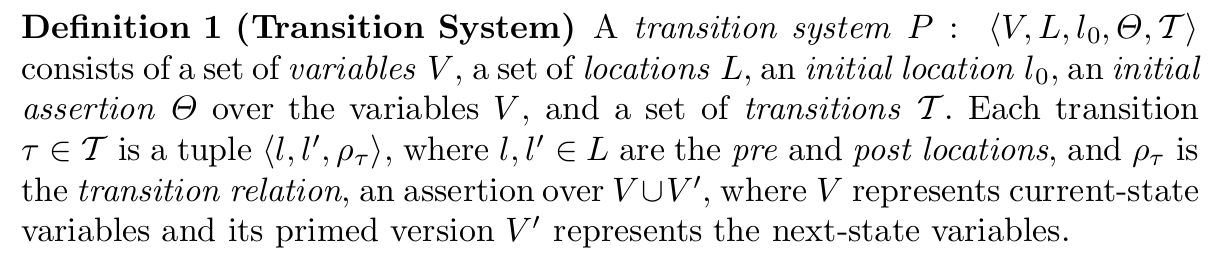
\includegraphics[scale=0.25]{defts.png}

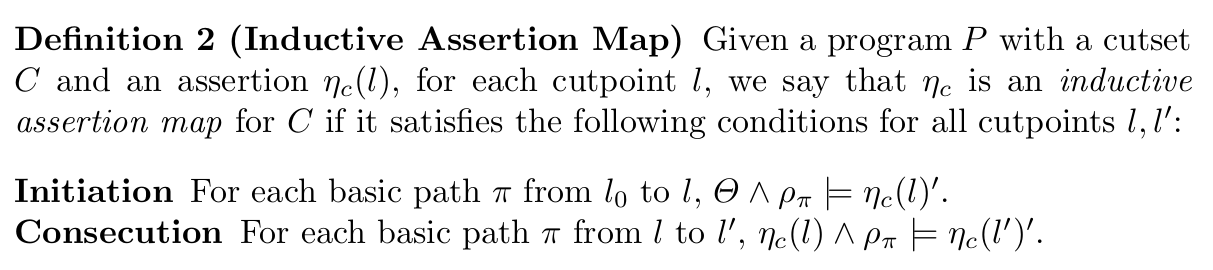
\includegraphics[scale=0.25]{defiam.png}
\end{center}

\end{frame}

\begin{frame}\frametitle{Linear Constraint}

\end{frame}

\begin{frame}\frametitle{Farkas' Lemma}
\begin{center}
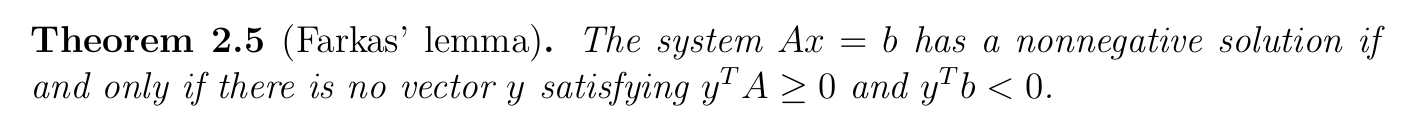
\includegraphics[scale=0.23]{farkas.png}
\end{center}

Intuitive understanding of farkas lemma.

\begin{center}

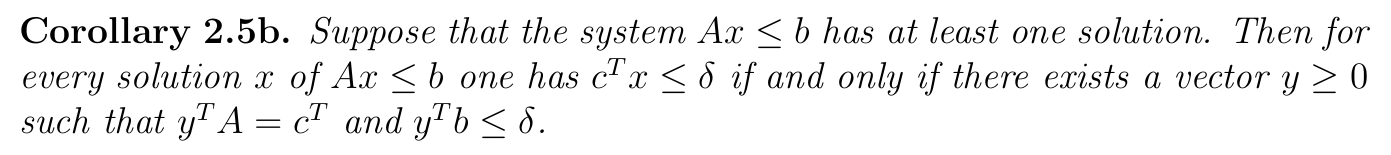
\includegraphics[scale=0.23]{farkasco.png}
\end{center}

\end{frame}

\begin{frame}\frametitle{Farkas' Lemma}
A better demonstration of the Corrollary.
\begin{center}
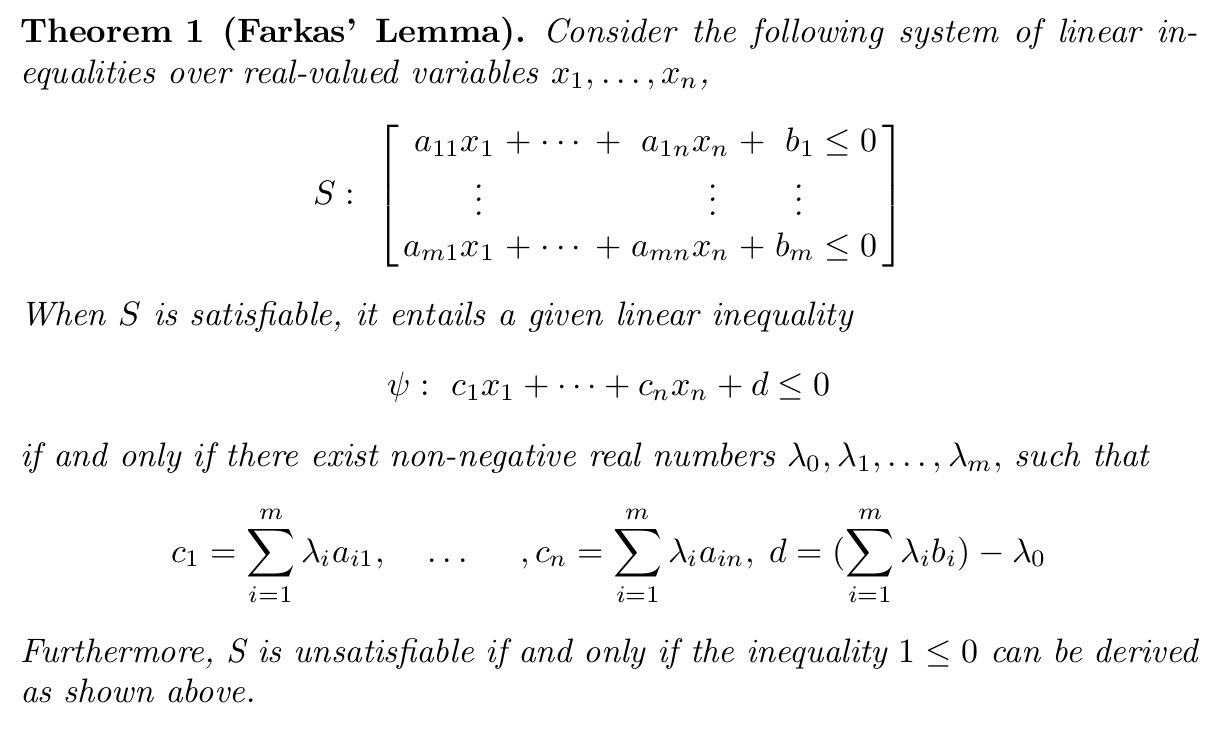
\includegraphics[scale=0.25]{fc.png}
\end{center}

\end{frame}

\begin{frame}\frametitle{Solving the Invariant of Transition System}

\end{frame}

\begin{frame}\frametitle{Quantifier Elimination}
\begin{itemize}
\item Exact quantifier elimination.

\item Under-approximate elimination approach			
\end{itemize}
\end{frame}
\end{document}